% REMEMBER: Write the thesis from the view of the reader. How would I like to READ the thesis?

\chapter{Testing Approach}

% - IO
% - parallel scripts
% - overhead

\section{General Approach}

\mnote{does knowing sprite and variable names make it grey-box?}
In this work, we propose a way to perform dynamic testing on Scratch programs.
Tests follow a black-bock approach and make use of a testing utility, which allows test code to interact with a running Scratch program.
% To enable dynamic testing for Scratch, we propose a black-bock approach with a testing utility, which allows test code to interact with a running Scratch program.

Because Scratch's parallel scripts and lack of code separation, would make white-box testing difficult,
we instead chose to ignore the internals and only focus on the input and output of the program.
Of course, this raises the question of how to access Scratch's IO.
Since Scratch's input usually consists of mouse and keyboard input, and its output consists of visual animations and sound,
they are not easily accessible in a programmable way.
To overcome this challenge, we developed a testing utility, which acts as a wrapper around Scratch.
It interacts with Scratch's virtual machine instead of its GUI in order to automate the IO.
This utility offers a programmable interface for Scratch, which makes black-box testing possible.

% Therefore, we only concern ourselves with ...

% We are going to deal with this problem by creating a wrapper around Scratch,
% which can be used to simulate input and access information about the sprites which make up the output.
% Tests can then use methods, which the wrapper provides, instead of manually interacting with the Scratch program.

% Therefore, additional computations by the testing procedure must be fast enough to avoid interfering with the program under test.

\mnote{TODO: better captions}
\begin{figure}[h]
    \centering

    \begin{subfigure}[b]{\textwidth}
        \centering
        \tikzset{>=latex,
                 put/.style={draw, text width=2.5cm, minimum height=2.2cm, minimum width=3.5cm, text centered, fill=black!90, text=white, rounded corners},
                  vm/.style={draw, minimum height=3.5cm, minimum width=6.0cm, fill=white, rounded corners},
                 gui/.style={draw, minimum height=4.7cm, minimum width=7.0cm, fill=blue!20, rounded corners},
            arrowtxt/.style={text width=3.3cm, midway}}

         \begin{tikzpicture}[scale=0.8, every node/.style={scale=0.8}]
            \begin{scope}[on background layer]
                \node[gui]     at (  5.9,  0.4) (gui)    {};
                \node[vm]      at (  5.9,  0.0) (vm)     {};
                \node[]        at ( -2.0,  0.4) (input)  {};
                \node[]        at ( 14.0,  0.4) (output) {};
            \end{scope}

            \node[put]         at (  5.9, -0.4) (put)    {\textbf{Program under test (Black box)}};
            \node[]            at (  5.9,  1.3) (vmtxt)  {\textbf{Scratch Virtual Machine}};
            \node[font=\large] at (  5.9, 2.25) (guitxt) {\textbf{Scratch GUI}};

            \path [draw, ->] (input) -- node [arrowtxt, above] {\textbf{Input}} (gui);
            \path [draw, ->] (gui)   -- node [arrowtxt, above] {\textbf{Output}} (output);
            \path [draw, ->] (input) -- node [arrowtxt, below] {Key presses, mouse movement, mouse clicks, etc.} (gui);
            \path [draw, ->] (gui)   -- node [arrowtxt, below] {Visual animations, audio, etc.} (output);
        \end{tikzpicture}
        \caption{Input and output of the Scratch GUI}
        \label{fig:input_and_output_of_the_scratch_gui}
    \end{subfigure}

    \bigskip

    \begin{subfigure}[b]{\textwidth}
        \centering
        \tikzset{>=latex,
                 put/.style={draw, text width=2.5cm, minimum height=2.2cm, minimum width=3.5cm, text centered, fill=black!90, text=white, rounded corners},
                  vm/.style={draw, minimum height=3.5cm, minimum width=6.0cm, fill=white, rounded corners},
                util/.style={draw, minimum height=4.7cm, minimum width=7.0cm, fill=green!20, rounded corners},
            arrowtxt/.style={text width=3.3cm, midway}}

         \begin{tikzpicture}[scale=0.8, every node/.style={scale=0.8}]
            \begin{scope}[on background layer]
                \node[util]    at (  5.9,  0.4) (util)    {};
                \node[vm]      at (  5.9,  0.0) (vm)      {};
                \node[]        at ( -2.0,  0.4) (input)   {};
                \node[]        at ( 14.0,  0.4) (output)  {};
            \end{scope}

            \node[put]         at (  5.9, -0.4) (put)     {\textbf{Program under test (Black box)}};
            \node[]            at (  5.9,  1.3) (vmtxt)   {\textbf{Scratch Virtual Machine}};
            \node[font=\large] at (  5.9,  2.2) (utiltxt) {\textbf{Testing Utility}};

            \path [draw, ->] (input) -- node [arrowtxt, above] {\textbf{Input}} (util);
            \path [draw, ->] (util)  -- node [arrowtxt, above] {\textbf{Output}} (output);
            \path [draw, ->] (input) -- node [arrowtxt, below] {Interface to simulate input} (util);
            \path [draw, ->] (util)  -- node [arrowtxt, below] {Interface to query information about sprites and variables} (output);
        \end{tikzpicture}
        \caption{Input and output of the testing utility}
        \label{fig:input_and_output_of_the_testing utility}
    \end{subfigure}

    \caption{Comparison of IO mechanisms}
    \label{fig:comparison_of_io_mechanisms}
\end{figure}

\section{Testing Procedure}

Automating Scratch allows us to write tests for Scratch in a unit-test-like fashion.
The utility can load and start the program before each test starts.
By doing this, we allow every test starts with a fresh instance of the program in the exact same situation.
The test code can then interact with the program in order to produce a desired situation and check how to program behaves through assertions.

\noindent Test code can use the testing utility to do the following:
\begin{itemize}
    \item \textbf{Simulate Input.}
        By simulating Scratch's main input methods, the test can control the tested program.
        The goal is to simulate a user interacting with the program.
        Therefore, this is the only way the test can manipulate the program.
        The possible input includes mouse movement, mouse button presses, keyboard key presses and entering answers to ask blocks.
    \item \textbf{Access Information.}
        \mnote{Explain how in the implementation chapter (objects)}
        The testing utility can be used to access sprites and variables of the program.
        This makes it possible to gather information about anything, which is displayed on the stage.
        Analyzing Scratch's visual output would otherwise be very difficult.
        The provided sprite attributes include the sprite's position, rotation, size, current costume, speech bubble text, etc..
        The values of the program's variables can also be accessed.
        These variable values can usually be displayed to the user in Scratch's graphical output, and are commonly used in Scratch programs to convey information to the user.
    \item \textbf{Control the program execution.}
        The test is able to control when and for how long the program under test is run.
        In the beginning of the test, the program starts in a paused state with the green flag already pressed.
        The test can then run (resume) the program for a certain time, or until a condition is met.
        The green flag can also be pressed again in order to restart the program, which can, for example, be useful for testing programs, that use randomness.
    \item \textbf{Register Callbacks.}
        The test can register callbacks, which get called every time Scratch renders a new picture.
        This allows the test to track the information, which the user would normally see, while the program is running.
    \item \textbf{Register constraints.}
        By registering constraints, the test can define conditions that must always hold true.
        Constraints are done through special callbacks, which perform assertions.
        They are, like callbacks, checked every time Scratch renders a frame.
        For example, this can be used to define that a certain sprite always has to move right when the right arrow key is pressed.
\end{itemize}

However, the test can not:
\begin{itemize}
    \item \textbf{Directly manipulate sprite attributes.}
        The test should only interact with the program like a user would.
        Directly manipulating sprites or variables could result in unexpected behaviour of the program.
        Therefore, it does not make sense to directly manipulate sprites for testing Scratch.
    \item \textbf{Execute single scripts or blocks directly}.
        The block box approach does not allow knowledge about the code of the program.
        Executing single scripts could also lead to unexpected behaviour from the program, because the scripts could depend on other scripts, which run parallelly.
\end{itemize}

\section{Constraint-only Tests}%
\label{sec:constraint_only_tests}

- TODO: when constraints are checked can't be clear here, a different implementation could allow constraints to be checked e.g. when a value is changed.

- Normally, tests would deliberately simulate input on the program, then perform some assertions
- Constraints open up a new approach to testing Scratch programs by only defining constraints instead of doing normal assertions
- In the end of the test, it has to be checked if the desired situation for the constraint occurred during the program execution
    - E.g. a constraint that describes the movement speed of a sprite will always hold if the sprite does not move at all
    - $\rightarrow$ The constraint need to be filtered
- This makes it possible to separate the checking of properties from the execution of the program
    - Checks are only done through constraints, which run in the background
    $\rightarrow$ This is independent from the program execution
    $\rightarrow$ The program can be controlled by arbitrary input, as long as the desired situation for the constraint(s) comes about
        - Deliberately simulated input
        - Manual user input
        - Random input ($\rightarrow$ well-suited for random input, because the test is independent from the source of input)
          Similar approaches have been used in other testing applications, e.g. QuickCheck \cite{quickcheck}

- Normal tests vs. constraint-only tests
    - Normal tests can be more granular $\rightarrow$ better for grading
    - Normal tests allow to write very short tests for things that can be checked fast
        - More difficult if everything is tested in a single constraint-only test
        $\rightarrow$ Better for continuous development, because it's easier to quickly execute just one test
    - Constraint-only test require more processing, constraints have to be checked between every step
    - Constraints can't fully replace normal assertions: some properties are better checked with normal assertions (e.g. a property only has to hold for one point in time)

\begin{figure}[h]
    \centering
    \begin{subfigure}[b]{.45\textwidth}
        \centering
        \tikzset{>=latex,
                 box/.style={draw, text width=4.3cm, minimum height=0.7cm, text centered, rounded corners},
                 num/.style={draw, circle, inner sep=0.6mm, text centered},
                   h/.style={fill=blue!10}}

        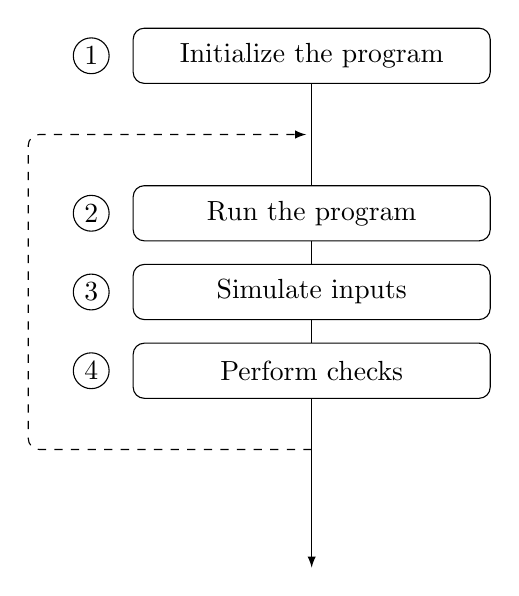
\begin{tikzpicture}
            \node[box] at ( 0.2,  5.0) (initialize) {Initialize the program};
            \node[box] at ( 0.2,  3.0) (run)        {Run the program};
            \node[box] at ( 0.2,  2.0) (inputs)     {Simulate inputs};
            \node[box] at ( 0.2,  1.0) (checks)     {Perform checks};

            \node[num] at (-2.6,  5.0) (one)   {1};
            \node[num] at (-2.6,  3.0) (two)   {2};
            \node[num] at (-2.6,  2.0) (three) {3};
            \node[num] at (-2.6,  1.0) (four)  {4};

            \draw[->]
                   (initialize)
                -- (run)
                -- (inputs)
                -- (checks)
                -- ( 0.2, -1.5);

            \draw[shorten >= 2pt, rounded corners, dashed, ->]
                   ( 0.2,  0.0)
                -- (-3.4,  0.0)
                -- (-3.4,  4.0)
                -- ( 0.2,  4.0);
        \end{tikzpicture}

        \caption{Normal Test Procedure}
        \label{fig:normal_test_procedure}
    \end{subfigure}
    \begin{subfigure}[b]{.45\textwidth}
        \centering
        \tikzset{>=latex,
                 box/.style={draw, text width=4.3cm, minimum height=0.7cm, text centered, rounded corners},
                 num/.style={draw, circle, inner sep=0.6mm, text centered},
                   h/.style={fill=blue!10}}

        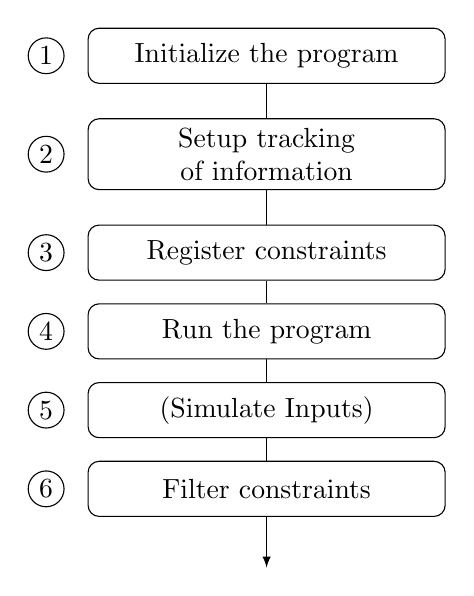
\begin{tikzpicture}
            \node[box] at ( 0.2,  5.5)  (initialize)  {Initialize the program};
            \node[box] at ( 0.2,  4.25) (tracking)    {Setup tracking of information};
            \node[box] at ( 0.2,  3.0)  (constraints) {Register constraints};
            \node[box] at ( 0.2,  2.0)  (run)         {Run the program};
            \node[box] at ( 0.2,  1.0)  (inputs)      {(Simulate Inputs)};
            \node[box] at ( 0.2,  0.0)  (filter)      {Filter constraints};

            \node[num] at (-2.6,  5.5)  (one)   {1};
            \node[num] at (-2.6,  4.25) (two)   {2};
            \node[num] at (-2.6,  3.0)  (three) {3};
            \node[num] at (-2.6,  2.0)  (four)  {4};
            \node[num] at (-2.6,  1.0)  (five)  {5};
            \node[num] at (-2.6,  0.0)  (six)   {6};

            \draw[->]
                   (initialize)
                -- (tracking)
                -- (constraints)
                -- (run)
                -- (inputs)
                -- (filter)
                -- ( 0.2, -1.0);
        \end{tikzpicture}

        \caption{Constraint-only Test Procedure}
        \label{fig:constraint_only_test_procedure}
    \end{subfigure}
    \caption{Comparison of the procedure of normal tests and constraint-only tests}
    \label{fig:comparison_of_the_procedure_of_normal_tests_and_constraint_only_tests}
\end{figure}

\section{Advantages and Disadvantages}

=== Shortcomings of this approach
- Scratch projects need to be well defined to be tested
    - Can take the creativity out of the process, but can also give the students a guide to follow, which helps them to not get stuck on one problem
    - Students can test their programs with the test suite beforehand on their own to verify their programs
    - Problem: might incentivize students to try to cheat the tests
        $\rightarrow$ Automated testing should only be used in conjunction with static analysis, manual analysis, or random secret tests
        (static analysis should easily show anomalies on the projects)
- Scratch programs can be pretty inconsistent
    - Some programs may only sometimes work and other times not
    $\rightarrow$ They may or may not pass the test

=== Advantages
- Allows the full range of Scratch functionality
    - ITCH only allows textual input and output, greatly limiting the possible functionality of tested programs
- Tests are easily understandable since they use the program like a normal user would
    - Students can test their programs with the test suite beforehand on their own to verify their programs
        $\rightarrow$ Students can easily receive feedback and will change their programs according to the tests
        $\rightarrow$ Incentivizes students to ask for help if they can't progress, because the test clearly shows that there is a problem
